\section{A Classification Framework for SoTS}\label{sec:literature-review-classification}
To organize how DTs and SoS concepts are combined, we developed a classification framework grounded in classical SoS theory~\cite{maier1998architecting, maier2014role} and foundational DT concepts~\cite{kritzinger2018digital}. Using a mixed sample-case generalization approach~\cite{wieringa2015six}. Studies from the corpus (\secref{sec:literature-review-study-design}) were decomposed into architectural abstractions to identify recurring patterns.

\subsection{Core Elements}
The framework identifies several core architectural elements. A \textit{System} represents the fundamental building block of a SoS and may be hierarchically composed of other systems. In SoTS, systems may be associated with \textit{Physical Twins} and corresponding \textit{Digital Twins}, where the DT maintains a digital representation of system state through computational models and data-driven updates \cite{kritzinger2018digital}. A key distinction concerns coupling. SoS constituents typically interact through relatively \textit{weak coupling}, allowing independent operation and decision-making, whereas DTs maintain \textit{strong coupling} with their physical counterparts through continuous data exchange and feedback.

Some architectures also introduce a coordinating element responsible for system-level decision making. This \textit{controller} role may be implemented by a higher-level DT or supervisory component that aggregates information and coordinates behavior across multiple constituents.

These elements form the basis for identifying recurring SoTS architectural patterns discussed in the following sections.

\subsection{Instances}
\begin{figure}[H]
\centering

% --- Row 1 ---------------------------------------------------
\subfloat[Directed SoTS]{%
    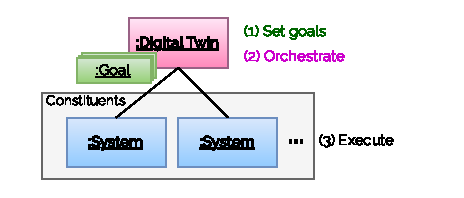
\includegraphics[trim={0.66cm 0.25cm 1.1cm 0.25cm},clip,
    width=0.4\linewidth]{figures/Literature Review/framework/instances/directed.pdf}}
\hfill
\subfloat[Acknowledged SoTS]{%
    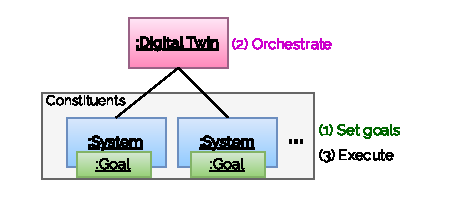
\includegraphics[trim={0.66cm 0.25cm 1.1cm 0.25cm},clip,
    width=0.4\linewidth]{figures/Literature Review/framework/instances/acknowledged.pdf}}
\\[1.2em]

% --- Row 2 ---------------------------------------------------
\subfloat[Collaborative SoTS]{%
    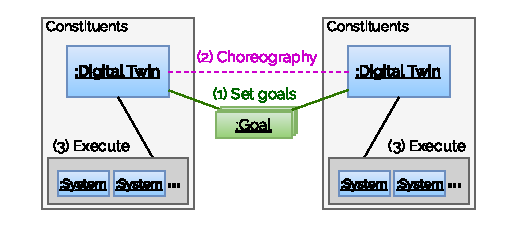
\includegraphics[trim={0.66cm 0.25cm 0.75cm 0.25cm},clip,
    width=0.4\linewidth]{figures/Literature Review/framework/instances/collaborative.pdf}}
\hfill
\subfloat[Virtual SoTS]{%
    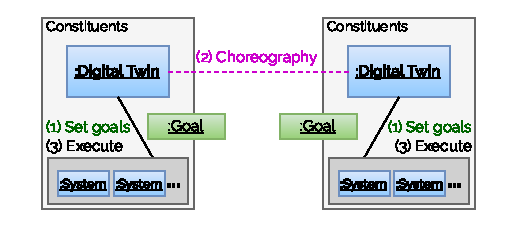
\includegraphics[trim={0.66cm 0.25cm 0.75cm 0.25cm},clip,
    width=0.4\linewidth]{figures/Literature Review/framework/instances/virtual.pdf}}
\\[1.2em]

% --- Row 3 ---------------------------------------------------
\subfloat[System of Specialized DTs]{%
    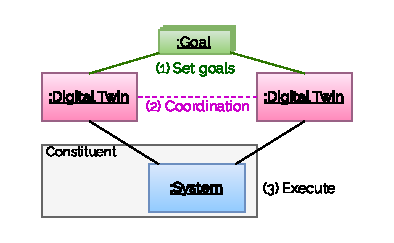
\includegraphics[trim={0.66cm 0.25cm 0.50cm 0.25cm},clip,
    width=0.4\linewidth]{figures/Literature Review/framework/instances/domainspec.pdf}}
\hfill
\subfloat[System of Specialized DTs and Specialized Systems]{%
    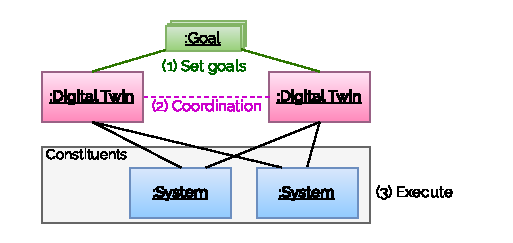
\includegraphics[trim={0.66cm 0.25cm 0.75cm 0.25cm},clip,
    width=0.4\linewidth]{figures/Literature Review/framework/instances/domainspec2.pdf}}

\caption{Overview of the six architectural styles observed in SoTS}
\label{fig:sots-architectures}
\end{figure}

Six recurring SoTS architectures were identified (\figref{fig:sots-architectures}). Four align with \citet{maier1998architecting}'s canonical SoS types---directed, acknowledged, collaborative, and virtual---while two reflect DT-specific specializations. Each architecture represents a different way of organizing control, goals, and coordination between DTs and their physical systems. \textbf{Directed SoTS} follow a hierarchical structure, where a central DT sets system-wide goals and coordinates the behaviour of other DTs. Constituent systems remain independent, but their actions are guided by the central controller. \textbf{Acknowledged SoTS} also include a central DT, but it coordinates rather than controls. Each DT keeps its own local goals, and system behaviour is shaped through coordination between the central DT and the constituents. \textbf{Collaborative SoTS} remove the central controller entirely. DTs coordinate directly with each other, working together to achieve shared goals through peer-to-peer interaction. \textbf{Virtual SoTS} go further, with fully autonomous DTs that define their own goals. They form and break connections dynamically, and coordination emerges based on current context and local decisions.

Two additional architectures arise from DT specialization. A \textbf{System of Specialized DTs} consists of multiple DTs representing different aspects of the same physical system. These DTs must coordinate to keep their views consistent and support joint decisions. The broader \textbf{System of Specialized DTs and Systems} extends this idea across multiple systems, where specialized DTs coordinate across system boundaries using shared models or standards instead of a central controller. Together, these six architectures show how SoTS organize control, coordination, and autonomy in DT-based systems.